% =============================================================================
%  Bachelor Thesis — Universität Konstanz Style
%  Konstanz Bus Network Analysis (2019 vs 2025)
%  Compatible with TinyTeX minimal installation
% =============================================================================
\documentclass[12pt,a4paper,oneside]{report}

% ---------------------------------------------------------------------------
%  Encoding & language
% ---------------------------------------------------------------------------
\usepackage[utf8]{inputenc}
\usepackage[T1]{fontenc}
\usepackage{lmodern}

% ---------------------------------------------------------------------------
%  Page geometry
% ---------------------------------------------------------------------------
\usepackage[
  left=3cm,
  right=2.5cm,
  top=2.5cm,
  bottom=2.5cm,
  bindingoffset=0.5cm
]{geometry}

% ---------------------------------------------------------------------------
%  Line spacing (1.5)
% ---------------------------------------------------------------------------
\linespread{1.3}

% ---------------------------------------------------------------------------
%  Universität Konstanz corporate colours
% ---------------------------------------------------------------------------
\usepackage{xcolor}
\definecolor{unikn-seeblau}{RGB}{0,169,224}
\definecolor{unikn-darkblue}{RGB}{0,90,148}
\definecolor{unikn-petrol}{RGB}{0,110,101}
\definecolor{unikn-grey}{RGB}{155,155,155}

% ---------------------------------------------------------------------------
%  Graphics, tables, maths
% ---------------------------------------------------------------------------
\usepackage{graphicx}
\usepackage{booktabs}
\usepackage{tabularx}
\usepackage{longtable}
\usepackage{amsmath,amssymb}
\usepackage{float}

% ---------------------------------------------------------------------------
%  Bibliography (natbib + apalike)
% ---------------------------------------------------------------------------
\usepackage{natbib}
\bibliographystyle{apalike}

% ---------------------------------------------------------------------------
%  Hyperlinks
% ---------------------------------------------------------------------------
\usepackage[
  colorlinks=true,
  linkcolor=unikn-darkblue,
  citecolor=unikn-darkblue,
  urlcolor=unikn-seeblau,
  bookmarksopen=true,
  pdfstartview=FitH
]{hyperref}

% ---------------------------------------------------------------------------
%  Custom commands
% ---------------------------------------------------------------------------
\newcommand{\unikn}{Universit\"{a}t Konstanz}
\newcommand{\pspace}{\textit{P}-space}

% ═══════════════════════════════════════════════════════════════════════════════
%  DOCUMENT
% ═══════════════════════════════════════════════════════════════════════════════
\begin{document}

% ---------------------------------------------------------------------------
%  Title page — Universität Konstanz style
% ---------------------------------------------------------------------------
\begin{titlepage}
  \centering

  % University logo placeholder – replace with actual logo file
  \vspace*{1cm}
  % \includegraphics[width=6cm]{unikonstanz-logo.pdf}

  {\Large\scshape\color{unikn-seeblau} Universit\"{a}t Konstanz}\\[0.3cm]
  {\large Fachbereich Politik- und Verwaltungswissenschaft}\\[0.15cm]
  {\large Department of Politics and Public Administration}

  \vspace{2cm}
  \rule{\textwidth}{1.5pt}\\[0.5cm]
  {\huge\bfseries\color{unikn-darkblue}
    How Is the Public Transport Network\\[0.25cm]
    in Konstanz Structured?}\\[0.4cm]
  {\Large\color{unikn-darkblue}
    Hubs, Bottlenecks, and Network Change\\
    Between the 2019 and 2025 Timetable Versions}\\[0.3cm]
  \rule{\textwidth}{1.5pt}

  \vspace{1.5cm}
  {\large Bachelor Thesis}\\[0.5cm]
  {\large Submitted in Partial Fulfilment of the Requirements for the Degree of}\\[0.2cm]
  {\large\textbf{Bachelor of Arts (B.\,A.)}}

  \vfill

  \begin{tabular}{rl}
    \textbf{Author:}       & Levi \\[0.15cm]
    % \textbf{Matrikelnr.:}  & 01/XXXXXX \\[0.15cm]
    \textbf{First examiner:}  & Prof.\,Dr.\ [Name] \\[0.15cm]
    \textbf{Second examiner:} & [Name] \\[0.15cm]
    \textbf{Date:}            & \today \\
  \end{tabular}

  \vspace{1.5cm}
\end{titlepage}

% ---------------------------------------------------------------------------
%  Abstract
% ---------------------------------------------------------------------------
\chapter*{Abstract}
\addcontentsline{toc}{chapter}{Abstract}

This thesis examines how the public bus network in Konstanz is structured, which hubs and bottlenecks can be identified, and how these features change between two timetable versions (2019 and 2025).
The study models the network as a transfer-free reachability graph in which two stops are connected if they can be reached on the same bus line without changing buses.
Timetable information was manually extracted from the official Stadtbus Konstanz timetable booklet for a typical weekday service snapshot in May around midday.
Network measures are computed for each year and compared.

The results show a small increase in overall transfer-free connectivity from 2019 to 2025, with stops rising from 107 to 108 and undirected connections rising from 1,746 to 1,834.
Among stops present in both years, 233 direct stop pairs are newly connected in 2025 while 177 direct pairs are removed, indicating substantial rewiring beneath a stable core.
Central hubs remain largely unchanged, with Bahnhof, Konzilstr./Theater, Sternenplatz, and Z\"{a}hringerplatz consistently ranking highest by degree and betweenness.
Maximum betweenness decreases from 855.64 to 757.99, suggesting a modest reduction in extreme dependency on a single structural bottleneck.
A robustness check based on node-removal simulations also indicates slightly higher robustness in 2025 under the transfer-based network model.
Overall, the findings indicate a stable backbone combined with redistribution of transfer-free accessibility across stops, producing clear winners and losers.

\medskip
\noindent\textbf{Keywords:} public transport, network analysis, adjacency matrix, hubs, bottlenecks, Konstanz, timetable comparison

% ---------------------------------------------------------------------------
%  Table of contents
% ---------------------------------------------------------------------------
\tableofcontents
\clearpage

% ═══════════════════════════════════════════════════════════════════════════════
%  CHAPTER 1 — Introduction
% ═══════════════════════════════════════════════════════════════════════════════
\chapter{Introduction}\label{ch:introduction}

\section{Problem and motivation}\label{sec:problem}

Public transport networks are often experienced through a simple everyday question.
Can I get from where I am to where I want to go without changing vehicles, and if not, how complicated does the trip become?
Behind this practical perspective sits a system with a measurable structure.
Stops and stations form the nodes of a network, and service patterns create connections that determine how flows are channelled through a city.
Network analysis provides a way to describe this structure systematically and to identify which parts of the system act as central hubs, and which parts constitute bottlenecks that constrain connectivity \citep{barthelemy2011}.
A related strand of research shows that the robustness of public transport networks depends strongly on how connectivity is distributed across the network, because systems that rely heavily on a small number of key nodes can be more vulnerable to disruptions and rerouting costs \citep{derrible2010}.

Konstanz offers a particularly relevant case for such an analysis.
It is neither a large metropolitan transit system nor a trivial small network.
Instead, it is a medium-sized urban setting whose bus services connect residential areas, employment centres, and highly frequented destinations such as the city centre and the university.
In such contexts, planning constraints and limited redundancy can shape network structure in ways that differ from the large-city cases that dominate much of the literature \citep{cipriani2019}.
This thesis therefore uses Konstanz as a case study to connect practical concerns about service design with theoretical concepts from transport network analysis.

The thesis is also motivated by change.
Timetables are not static, and service reforms can alter not only individual routes but also the network properties that emerge from the full set of services.
Comparing two timetable versions provides a concrete before-and-after design that makes network change observable.
In this thesis, two snapshots of the Konstanz bus network are compared, one based on the 2019 timetable and one based on the 2025 timetable.
The empirical focus is deliberately placed on direct connectivity without transfers, because transfer-free travel is both highly salient for passengers and analytically transparent as a network relation.

\section{Research question and objectives}\label{sec:research-question}

The overarching research question is:

\begin{quote}
\emph{How is the public transport network in Konstanz structured, which hubs and bottlenecks can be identified, and how do these features change between the 2019 and 2025 timetable versions?}
\end{quote}

This question is addressed through a network representation in which stops are nodes and a connection between two stops exists if they are reachable within the same bus service pattern without changing buses.
This choice is inspired by research that emphasises the importance of service patterns and network structure for travel efficiency in public transport systems \citep{gallotti2014} and by work that situates public transport in a broader context of multimodal and multilayer network thinking, even if the present thesis uses a simpler, bus-focused representation for feasibility and interpretability \citep{alessandretti2022,artime2022}.

The independent variable in the comparison is the timetable version, operationalised as the 2019 versus 2025 network snapshot.
The dependent variables are network outcomes derived from the constructed graphs.
These include (1)~direct connection presence between pairs of stops in the adjacency representation, (2)~node-level indicators of hub and bottleneck status such as degree and betweenness centrality, and (3)~global network characteristics such as density, clustering, and shortest-path-based measures that capture overall connectivity \citep{barthelemy2011,derrible2010}.

More specifically, the thesis pursues three objectives.
First, it provides a descriptive account of the Konstanz bus network structure in each year by quantifying connectivity and identifying central nodes.
Second, it evaluates whether the hub hierarchy and bottleneck structure remain stable or shift between 2019 and 2025, which links directly to the idea that some networks concentrate flows around key nodes while others distribute connectivity more evenly \citep{derrible2010}.
Third, it translates the year-to-year comparison into an interpretable change perspective by distinguishing connections that are newly available without transfers from those that disappear, thereby connecting network analysis to a user-relevant notion of accessibility in the everyday sense of transfer-free reachability.

Importantly, this thesis does not aim to provide a full operational evaluation of public transport quality, and it does not model demand, waiting times, or service frequency in detail.
Instead, it focuses on the structural implications of service patterns and their change over time.
This emphasis keeps the analysis feasible at bachelor-thesis scope while still enabling theoretically meaningful statements about hubs, bottlenecks, and the consequences of network rewiring.

\section{Structure of the thesis}\label{sec:structure}

Chapter~\ref{ch:literature} reviews the relevant literature and develops the theoretical framework.
It introduces public transport as a spatial network \citep{barthelemy2011}, discusses hubs and bottlenecks as structural features linked to vulnerability and robustness \citep{derrible2010}, and connects the analysis to work on efficiency and service-pattern-based mobility networks \citep{gallotti2014}, including a brief positioning within the broader field of multimodal and multilayer transport networks \citep{alessandretti2022,artime2022}.
The chapter then derives the research gap and clarifies how a medium-sized case such as Konstanz contributes to a literature that often focuses on larger systems \citep{cipriani2019}.

Chapter~\ref{ch:data} describes the data and operationalisation.
It explains how the two timetable versions are transformed into a harmonised stop set and how direct connections without transfers are defined to construct adjacency-based network snapshots for 2019 and 2025.

Chapter~\ref{ch:methods} presents the methods.
It details the construction of the networks, the computation of descriptive and centrality measures, and the comparison strategy used to classify connections as unchanged, newly gained, or removed between the two years.

Chapter~\ref{ch:results} reports the results.
It presents the network metrics for each timetable version, identifies hubs and bottlenecks, and shows where the largest gains and losses in transfer-free connectivity occur.

Chapter~\ref{ch:discussion} discusses the findings in relation to the literature and practical relevance, and it addresses limitations stemming from the chosen representation and the scope of the analysis.

Chapter~\ref{ch:conclusion} concludes by answering the research question and outlining possible extensions, including more time-sensitive representations, frequency weighting, or integration of additional modes where appropriate.

% ═══════════════════════════════════════════════════════════════════════════════
%  CHAPTER 2 — Literature review
% ═══════════════════════════════════════════════════════════════════════════════
\chapter{Literature review and theoretical framework}\label{ch:literature}

\section{Public transport as a networked spatial system}\label{sec:network-system}

A core idea of network analysis is that complex systems can be represented as graphs consisting of nodes and edges.
In transport contexts, nodes commonly represent stops or stations, while edges represent some form of connectivity, such as physical links, scheduled services, or the ability to travel between two points within the system.
This abstraction enables a systematic description of structure, including how connectivity is distributed, how concentrated or decentralised the system is, and which parts of the network constrain movement \citep{barthelemy2011}.

For public transport networks, the choice of representation is not merely technical, because it determines what the network measures mean.
A representation that connects only consecutive stops captures the physical adjacency of the service pattern, while a representation that connects all stops that can be reached within the same vehicle captures transfer-free reachability.
This representation is particularly relevant for questions of perceived convenience, since transfers are commonly associated with an additional perceived burden and can affect generalised cost beyond in-vehicle travel time \citep{iseki2009}.
\citet{gallotti2014} show that timetable-based network representations can be used to study the efficiency of urban mobility, and they highlight that network structure matters for the detours and constraints travellers experience.
This provides a direct motivation for focusing on transfer-free connectivity as an interpretable unit of analysis.

Public transport networks can be represented in several standard network spaces, and each representation encodes a different operational meaning.
In \textit{L}-space, edges connect consecutive stops along a route, so shortest paths reflect stop-to-stop progression along lines.
In \pspace{}, two stops are connected if they are served by at least one common line, so shortest paths approximate transfer requirements rather than physical adjacency.
A related bipartite representation, often called \textit{B}-space, connects stops to routes as two node types and allows projecting either a stop graph or a route graph depending on the research question.
Because these representations can yield different values for clustering, path length, and hub prominence, stating the chosen space explicitly is essential for interpretation and comparability across studies \citep{shanmukhappa2019}.

This thesis uses a \pspace{} stop graph to operationalise transfer-free connectivity, where an edge indicates that two stops are jointly served by at least one line.
In this representation, graph distance is interpretable in behavioural terms.
A path length of~1 corresponds to a trip with zero transfers, and a path length of~$d$ corresponds to approximately $d-1$ transfers under the simplifying assumption that each edge can be traversed by staying on a single line.
A known consequence of \pspace{} is clique-like densification induced by multi-stop routes, which increases clustering and can compress diameters relative to \textit{L}-space.
The implication is that network statistics should be interpreted as transfer structure rather than as street-level adjacency or geometric proximity \citep{shanmukhappa2019,zhang2025}.

In addition, public transport systems are often described as multimodal networks, because multiple services and modes collectively shape mobility.
Research on multimodal and multilayer transport networks emphasises that modes can be conceptualised as layers linked through interchange points, and that interdependencies across layers can matter for performance and vulnerability \citep{alessandretti2022,artime2022}.
In practice, however, a thesis must balance theoretical richness with feasibility.
The present study therefore adopts a deliberately simplified approach that focuses on the bus network of Konstanz.
It remains conceptually aligned with multimodal perspectives by treating the network as a service-based mobility system and by emphasising the role of transfer-free connectivity, but it does not implement a full multilayer modelling framework.

\section{How network analysis is applied in public transport research}\label{sec:applications}

Network analysis has become a widely used tool for studying public transport systems because it translates complex service structures into a common analytical language that allows systematic comparison, diagnosis, and evaluation.
This section reviews the main ways in which researchers and practitioners apply network-theoretic methods to transit systems, in order to position the present thesis within this broader landscape of applied use.

A first major application area is \emph{structural diagnosis and benchmarking}.
Researchers use network metrics such as density, clustering, diameter, and centrality distributions to characterise the overall shape of a transit system and to compare it against other cities or against theoretical network models.
For example, \citet{derrible2010} analyse 33~metro networks worldwide using degree distributions, clustering coefficients, and robustness indicators, producing a comparative typology that distinguishes hub-dominated systems from more evenly distributed ones.
Such benchmarking studies help planners understand where a given system stands relative to peers and what structural trade-offs it embodies, for instance whether a network prioritises directness over coverage, or whether connectivity is concentrated around a small number of interchange nodes.

A second application area is \emph{vulnerability and disruption analysis}.
Network analysis provides a structured way to ask what happens when parts of a transit system fail.
By simulating the removal of stops, stations, or entire lines and measuring how connectivity degrades, researchers can identify critical points whose failure would disproportionately affect the rest of the system.
\citet{albert2000} demonstrate this logic for complex networks in general, showing that scale-free networks are robust to random failures but fragile under targeted attack on hubs.
In the transit context, this translates into practical questions: which stations, if closed for construction or disrupted by an event, would cause the largest increase in travel time or the largest loss of reachable destinations?
Studies applying this approach have informed infrastructure prioritisation and contingency planning in cities ranging from large metro systems to regional bus networks \citep{derrible2010,cicchini2024}.

A third application concerns \emph{service change evaluation}.
When transit agencies redesign routes, add new lines, or restructure timetables, network analysis offers a before-and-after framework to quantify what changed structurally.
Rather than relying solely on ridership data, which may take months to stabilise after a reform, network metrics can immediately describe whether a redesign increased or decreased connectivity, whether it shifted the hub hierarchy, and which areas gained or lost direct accessibility.
\citet{cats2017} demonstrate this approach by analysing a major bus-network redesign in Stockholm, showing that topological indicators can capture structural effects of service reforms that are not immediately visible in aggregate ridership figures.
This diagnostic use is particularly relevant for the present thesis, which applies exactly this logic to the Konstanz timetable change between 2019 and 2025.

A fourth area is \emph{accessibility and equity assessment}.
Network-based accessibility measures can reveal how unevenly connectivity is distributed across a city.
If certain neighbourhoods have high degree centrality while others are peripheral with long shortest paths, the network structure reflects spatial inequality in service provision.
\citet{welch2013} use network topology to evaluate how well transit systems serve different population groups and how graph-based accessibility relates to socio-economic outcomes.
Closeness centrality, for instance, can serve as a proxy for how easily residents of different areas can reach the rest of the system, and changes in closeness across timetable versions can indicate whether reforms reduce or reinforce existing disparities.
Although the present thesis does not perform a full equity analysis, the winners-and-losers comparison at the stop level connects to this tradition by identifying which locations gain and which lose transfer-free reachability.

A fifth application is \emph{network design and optimisation}.
Transit network design research uses graph-theoretic objectives, such as minimising average path length or maximising coverage subject to resource constraints, to propose or evaluate route configurations.
\citet{cipriani2019} show that such optimisation is especially challenging in small and medium-sized cities, where limited fleet size and demand density constrain feasible designs.
While the present thesis does not optimise routes, the structural metrics it computes, such as density, clustering, and the distribution of centrality, are the same quantities that design models seek to improve.
The descriptive analysis can therefore be read as an input to or a diagnostic check on planning decisions.

Finally, network analysis is used to study \emph{temporal dynamics and resilience over time}.
Transit networks are not static objects; they evolve as timetables change, new infrastructure is built, or services are restructured.
Tracking how network properties change across multiple snapshots can reveal long-term trends in centralisation, redundancy, or fragmentation.
\citet{gallotti2014} emphasise that efficiency in urban mobility depends on the evolving interplay between network structure and travel patterns.
This temporal perspective motivates the two-snapshot comparison in the present thesis and connects it to a broader research agenda on how public transport networks adapt over time.

In summary, network analysis serves public transport research as a versatile diagnostic toolkit.
It is used to benchmark systems, identify vulnerabilities, evaluate reforms, assess spatial equity, inform design, and track change over time.
The present thesis draws primarily on the vulnerability, service-change evaluation, and temporal-comparison applications, while using the same structural metrics that underpin benchmarking and design research.

\section{Network structure, hubs, and centrality}\label{sec:hubs-centrality}

Within network analysis, hubs are typically understood as nodes that are structurally important because they connect many other nodes, or because they lie on a large share of shortest paths.
Centrality measures provide operational definitions of such importance.
Degree centrality captures how many direct connections a node has.
Betweenness centrality captures how frequently a node lies on shortest paths between other nodes, which often indicates that the node channels movement through the system.
Closeness centrality captures how near a node is to all others in terms of shortest-path distance, which can be interpreted as a measure of overall accessibility from that node to the rest of the network \citep{barthelemy2011}.

In a \pspace{} transfer-free reachability graph, standard centrality measures are explicitly service-oriented.
Degree captures how many other stops can be reached without a transfer, which reflects the breadth of direct access provided by overlapping lines at a stop.
Betweenness highlights transfer mediation, because high-betweenness nodes lie on many shortest paths that correspond to low-transfer itineraries.
Closeness reflects how quickly a stop can reach the rest of the system in terms of transfers, which aligns with transfer friction as a key component of perceived travel cost.
This interpretation clarifies why centrality is informative in the present setting, while also keeping the distinction between structural importance and passenger volume explicit \citep{shanmukhappa2019,derrible2010}.

Recent evidence suggests that structurally central stops often, though not always, correspond to higher passenger demand, especially when frequency-weighted representations are used.
This does not imply that centrality is a substitute for demand data, but it supports using centrality rankings as a defensible way to identify candidate critical stops when detailed boarding counts are unavailable.
In this thesis, the robustness scenarios therefore treat top-ranked centrality nodes as plausible points of vulnerability, while interpreting results as structural vulnerability rather than as direct statements about ridership impacts \citep{sfiligoj2025}.

A further implication is that hub structure may be relatively stable even when schedules change.
If the built environment and major demand anchors remain similar, certain central stops may retain their structural role across timetable revisions.
At the same time, local rewiring can create new hubs at secondary nodes or reduce the importance of previously central ones.
This motivates an explicit comparison across timetable versions.

\section{Bottlenecks, constraints, and robustness}\label{sec:bottlenecks}

Bottlenecks can be understood as nodes or edges whose removal would strongly disrupt connectivity, either by disconnecting parts of the network or by forcing large detours.
In network terms, bottlenecks are often associated with high betweenness and bridge-like positions between otherwise dense subnetworks.
A system that routes many shortest paths through a small number of nodes is structurally more concentrated and may be less robust to targeted disruptions \citep{derrible2010}.
This is especially relevant for public transport, where disruptions at key nodes can have cascading effects because passengers are re-routed to alternative services that may have limited capacity or may require additional transfers.

Robustness in networked systems is commonly studied by simulating disruptions and measuring how connectivity and efficiency degrade as nodes or edges are removed.
A standard distinction is between \emph{random failures}, which approximate uncorrelated local outages, and \emph{targeted attacks}, which remove the most central elements first and therefore test the system's dependence on hubs.
Across many complex networks, targeted removal fragments connectivity much faster than random failure, which makes hub identification central to vulnerability assessment \citep{albert2000}.
In public transport networks, this logic is often applied to stops as nodes and service connections as edges, with the largest connected component used as an indicator of whether a large share of the network remains mutually reachable \citep{derrible2010}.

Public transport disruptions can also act on routes as operational units rather than on single stops, and robustness depends on the extent to which passengers can reroute across overlapping services.
Route-based attack scenarios can reveal vulnerabilities that stop-based removal understates, especially in networks where many stops remain connected but redundancy collapses when entire lines are lost \citep{cicchini2024}.
In addition, multilayer and flow-based approaches show that structural robustness can diverge from functional robustness when passenger loads and transfer coupling drive cascading effects.
This motivates interpreting the stop-removal robustness analysis in this thesis as a structural baseline that is suitable for year comparison, while acknowledging that operational impacts could be stronger under route- or flow-based failure mechanisms \citep{hu2025}.

\section{Efficiency and transfer-free connectivity}\label{sec:efficiency}

Efficiency in public transport can be defined in many ways, including travel time, waiting time, number of transfers, or the detour relative to a straight-line route.
Even without modelling timetable frequencies or passenger demand, network structure can provide an analytically meaningful proxy for certain components of efficiency, particularly those related to transfers and detours.
\citet{gallotti2014} emphasise that the structure of multimodal mobility influences how efficiently travellers can navigate a city.
Building on this idea, the present thesis operationalises a simple and transparent concept of efficiency as transfer-free reachability.
Two stops are considered directly connected if a traveller can remain on the same bus service pattern to travel between them.
This yields an adjacency matrix of connections without transfers.

This representation makes the analysis interpretable, but it also implies certain limitations that are theoretically important to acknowledge.
The measure does not distinguish frequent connections from rare ones, and it does not capture time-dependent waiting costs.
It captures whether a transfer is necessary at all, not whether travel is fast or reliable.
Theoretically, this positions the measure closer to a structural accessibility concept, rather than a full generalised cost measure.
\citet{alessandretti2022} and \citet{artime2022} discuss how multimodal mobility research often emphasises richer representations, including layered structures and temporal dynamics.
The present thesis can therefore be viewed as a constrained but policy-relevant special case, in which transfer-free connectivity is treated as a central structural feature.

Transfer-free connectivity captures one dimension of service quality, but robustness and user experience also depend on redundancy, meaning the availability of multiple distinct ways to travel between origins and destinations.
A complementary concept is route diversity, which quantifies how many genuinely different itineraries exist and therefore how much flexibility passengers have when services or infrastructure are disrupted.
Framing transfer-focused connectivity alongside route diversity clarifies that structural improvements can arise either from more direct connections or from more diverse alternative paths, which provides a theoretical bridge between the metrics used here and broader planning goals related to resilience and reliability \citep{li2024}.

\section{The relevance of small and medium-sized city contexts}\label{sec:small-cities}

A further reason to study Konstanz is that public transport systems in small and medium-sized cities face design constraints that differ from those in large metropolitan contexts.
Service coverage, demand density, and operational resources shape feasible network designs, and limited redundancy can increase dependence on specific corridors or nodes.
Transit network design research for small and medium-sized cities highlights that planning often involves trade-offs under constraints, for example between coverage and directness, or between simplicity and connectivity \citep{cipriani2019}.
While the present thesis does not perform network design optimisation, it uses a similar lens to interpret structural outcomes.
In particular, if redundancy is limited, timetable changes may alter who benefits from transfer-free connectivity and where the network becomes more or less concentrated around key hubs.

\section{Research gap, contribution, and analytical expectations}\label{sec:research-gap}

The literature provides strong conceptual tools for analysing public transport as a network and for interpreting hubs, bottlenecks, efficiency, and robustness.
At the same time, empirical work often focuses on large systems or on static descriptions of a single network snapshot.
The contribution of this thesis is to apply these concepts to a medium-sized case and to introduce an explicit before-and-after comparison using two timetable versions, 2019 and 2025, as two network snapshots of the same city.
This design supports a clearer interpretation of change, because differences in network measures can be linked to a concrete intervention in the form of timetable revision, rather than to cross-city differences that may reflect broader contextual variation.

The analysis is guided by a small set of expectations derived from the literature.
First, if a timetable revision increases transfer-free connectivity, the network should become denser in the adjacency representation and should exhibit shorter average shortest paths, since more pairs can be reached without intermediate steps.
Second, if the revision reallocates connectivity rather than fundamentally restructuring the network, the identity of the most central hubs may remain stable while secondary hubs gain or lose importance.
Third, if the revision reduces structural concentration, extreme betweenness values may decrease, suggesting that the network becomes less dependent on a single critical bottleneck \citep{derrible2010}.
These expectations are not treated as strict hypotheses in a causal sense, because the thesis does not model demand or control for external changes.
They function as theory-informed lenses that connect the descriptive comparison to network concepts of concentration, accessibility, and vulnerability.

% ═══════════════════════════════════════════════════════════════════════════════
%  CHAPTER 3 — Data and operationalisation
% ═══════════════════════════════════════════════════════════════════════════════
\chapter{Data and operationalisation}\label{ch:data}

\section{Case and scope of the network}\label{sec:case}

This thesis analyses the public bus network serving the city of Konstanz and its directly connected districts and nearby localities that are part of the regular Stadtbus service area, including Wollmatingen, Dettingen, Wallhausen, Dingelsdorf, Oberdorf, Litzelstetten, and Mainau.
The analysis focuses on standard weekday operations.
Night services and weekend-only services are excluded, as are cross-border services towards Switzerland and the City Shuttle service.
The purpose of these scope decisions is to keep the network representation comparable across years and manageable within a bachelor thesis, while still covering the core everyday network relevant to most routine trips.

The empirical design is a before-and-after comparison between two timetable versions, one representing 2019 and one representing 2025.
The independent variable is the timetable version.
All network outcomes are computed separately for each year and then compared.

\section{Data sources and digitisation}\label{sec:data-sources}

The underlying data were manually extracted from the official printed timetable booklet used for the Konstanz bus network, commonly referred to as the \emph{Roter Arnold} timetable.
The timetable booklet is published by Stadtwerke Konstanz and is also made available as downloadable PDF timetables \citep{stadtwerke2019,stadtwerke2025}.

Because the timetable changes across weekends, holidays, and school periods, the dataset is constructed to represent a typical weekday service situation under normal operations.
For each year, the extraction focuses on a standard weekday in May and uses departures as close as possible to 12:00 to approximate a midday, normal-traffic snapshot.
This choice reduces the number of special-case variants that occur only during peak hours, school runs, or late evening periods, and it creates a consistent basis for comparison across 2019 and 2025.

The digitised data were converted into two CSV files, one for 2019 and one for 2025.
Each file stores the ordered structure of the network by listing directed connections between consecutive stops along each bus line.
In other words, each row represents an ordered pair of adjacent stops that appear next to each other in the line's stop sequence for the selected service snapshot, together with a line identifier.
The raw data were collected as ordered stop sequences for each bus line in the selected weekday snapshot.
The R script then transforms these sequences into a transfer-free connectivity network in which two stops are connected if they are served by the same line, meaning they are reachable without changing buses.
Importantly, this transfer-free representation is not limited to neighbouring stops in the timetable order, but connects any two stops that co-occur on at least one line pattern.

Because the timetable information was digitised manually, basic plausibility checks were applied.
The validation steps are described in Section~\ref{sec:plausibility}.

\section{Harmonising stop names and ensuring comparability}\label{sec:harmonising}

Stop names were harmonised across 2019 and 2025 to ensure that the same physical stop is represented by a consistent label.
The harmonisation procedure is described in Section~\ref{sec:harmonising-method}.
Year-to-year comparisons of pair-level change focus on the intersection of stops present in both years, as specified in Section~\ref{sec:pair-connectivity}.

The datasets also differ in their set of active lines.
In particular, line~9C exists in 2019 but not in 2025, reflecting a real service change.
This difference is treated as part of the timetable change captured by the independent variable rather than as a comparability problem.

\section{Constructing the transfer-free connectivity network}\label{sec:network-construction-data}

\subsection{Node definition}\label{sec:node-def-data}

Nodes are defined as bus stops.
Each unique harmonised stop name corresponds to one node in the network.

\subsection{Defining a connection without transfers}\label{sec:connection-def-data}

To analyse the Konstanz bus network in a way that is comparable across timetable versions, this study requires a clear operational definition of what constitutes a connection between two stops when transfers are excluded.
The analysis therefore focuses on transfer-free reachability, which captures whether two stops can be linked within the selected timetable snapshot without changing buses.
The formal network definition and construction rules used throughout the thesis are specified in Section~\ref{sec:transfer-free-def}.
In this representation, path length can be interpreted in terms of the minimum number of transfers required between stops.

\subsection{From stop sequences to an adjacency matrix}\label{sec:adj-matrix-data}

The digitised CSV files store adjacent stop pairs per line as an intermediate representation.
These sequences are converted into a binary stop-by-stop adjacency matrix as described in Section~\ref{sec:adj-matrix-construction}.
Although the CSV files list only consecutive stop pairs, they are used only as an intermediate representation to recover each line's served stop set.
The analytic network is then constructed as a transfer-free reachability graph: for each line, all stops served by that line are treated as mutually connected, so each line induces a complete subgraph over its stops (a clique).
As a consequence, density and clustering are expected to be higher than in a pure ``physical adjacency'' representation.

\section{Variables and outcomes}\label{sec:variables}

The independent variable is the timetable version (2019 vs.\ 2025).
Network outcomes at the pair, node, and global level are defined and operationalised in Section~\ref{sec:network-measures}.

\section{Summary of the analytic datasets}\label{sec:data-summary}

The digitised datasets represent two comparable network snapshots.
The 2019 network contains 107 stops, and the 2025 network contains 108 stops in the harmonised representation used for analysis.
Both networks form a single connected component in the undirected transfer-free representation, which means that all included stops are reachable from each other using a finite number of bus rides and transfers.
The year-to-year comparison therefore focuses on changes in connectivity patterns, hub prominence, and bottleneck structure rather than on the emergence of disconnected subsystems.

% ═══════════════════════════════════════════════════════════════════════════════
%  CHAPTER 4 — Methods
% ═══════════════════════════════════════════════════════════════════════════════
\chapter{Methods}\label{ch:methods}

\section{Analytical approach and software}\label{sec:approach}

The analysis follows a comparative network-analytic design.
Two network snapshots of the Konstanz bus system are constructed from manually digitised timetable information, one representing 2019 and one representing 2025.
All measures are computed separately for each snapshot and then compared.
The independent variable is the timetable version.
The dependent variables are structural properties of the resulting networks, including pair-level connectivity without transfers, node-level indicators of hub and bottleneck prominence, and global measures of connectivity and clustering.
This approach builds on established uses of network analysis for transport systems and on the interpretation of centrality and robustness concepts in transit networks \citep{barthelemy2011,derrible2010}.

All analyses were conducted in R \citep{rcore2025}.
Network construction, centrality measures, clustering, and shortest-path-based metrics were computed using standard graph routines.
In addition, permutation-based inference was used for node-level regression models relating betweenness centrality to structural predictors.
This approach avoids relying on classical OLS $p$-values, which can be misleading for network-derived outcomes.
Visualisations were generated with common plotting functions for matrix-style and network summary plots.

\section{Preprocessing, scope filters, and data validation}\label{sec:preprocessing}

\subsection{Scope filters}\label{sec:scope-filters}

To ensure comparability across years and to keep the analysis feasible, the datasets are restricted to a typical weekday service situation under normal operations.
Services that operate only at night or only on weekends were excluded, as were cross-border services towards Switzerland and the City Shuttle.
The geographic scope includes the core Konstanz service area and the regular lines connecting Konstanz to nearby localities that are part of the everyday network.
This scope definition is applied consistently to 2019 and 2025.

\subsection{Harmonising stop names}\label{sec:harmonising-method}

Stop names were standardised across the two datasets so that the same physical stop is represented by one consistent label in 2019 and 2025.
This harmonisation addresses spelling differences and known stop renamings.
The goal is to ensure that year-to-year differences in network measures reflect substantive timetable change rather than inconsistent naming.

\subsection{Basic plausibility checks}\label{sec:plausibility}

Because the timetable information was digitised manually, simple checks were used to detect transcription errors.
These checks verified that each line's extracted stop order forms a coherent sequence, that line identifiers are consistent, and that the stop set does not contain unintended duplicates created by formatting differences.
In addition, connectivity checks were run after network construction to confirm that the resulting network does not contain isolated nodes produced by data-entry mistakes.

\section{Network construction}\label{sec:construction}

A key methodological choice is how to translate timetable structure into a graph representation.
This thesis focuses on transfer-free connectivity, because it is directly interpretable and closely linked to perceived convenience.
The construction therefore proceeds in two steps: first recovering line-specific stop sequences, and then translating them into a transfer-free reachability relation between stop pairs.

\subsection{Nodes}\label{sec:nodes}

Nodes are bus stops.
The node set is defined as the unique set of harmonised stop names observed in each year.
The 2019 and 2025 node sets differ slightly, and this difference is treated as part of the substantive change between timetable versions.

\subsection{Defining transfer-free connectivity}\label{sec:transfer-free-def}

Two stops are considered connected if a passenger can travel between them while staying on the same bus, without changing buses.
In practical terms, this means that both stops appear on at least one common line service pattern in the selected weekday snapshot.
This operationalisation is consistent with a service-pattern perspective on transit networks and provides a simple structural proxy for an aspect of efficiency, namely avoiding transfers \citep{gallotti2014}.

The operational rule is deliberately not limited to neighbouring stops.
If a line serves a sequence of stops, then any pair of stops within that sequence is treated as mutually connected in the transfer-free sense.
This choice yields a dense adjacency structure, but it directly corresponds to the research focus.
The resulting graph should therefore be interpreted as a transfer-free reachability network, not as a physical street-adjacency network.

In the public transport network literature, this construction corresponds to a \pspace{} stop graph, where edges represent shared service by at least one line.
The \pspace{} perspective matches the study's focus on transfer-free reachability, because path length primarily reflects transfers rather than spatial adjacency.
At the same time, \pspace{} is known to induce dense subgraphs for multi-stop lines, which is why the analysis emphasises year-to-year comparison using the same construction rather than interpreting absolute values as physical travel proximity \citep{shanmukhappa2019,zhang2025}.

\subsection{Adjacency matrix construction}\label{sec:adj-matrix-construction}

For each timetable version, an adjacency matrix~$\mathbf{A}$ is constructed over the set of stops, where
\begin{equation}\label{eq:adjacency}
  A_{ij} =
  \begin{cases}
    1 & \text{if stops } i \text{ and } j \text{ are connected without transfers,}\\
    0 & \text{otherwise.}
  \end{cases}
\end{equation}
The matrix is built by iterating over all extracted line sequences.
For a given line, the set of served stops is taken, and all stop pairs within that set are marked as connected.

The analytic network is modelled as undirected.
A connection is coded as present if the stop pair is connected without transfers, independent of travel direction.
This choice treats transfer-free connectivity as a symmetric relationship between stops and simplifies interpretation of the adjacency matrix as a binary map of direct reachability.
The main limitation of this choice is that it abstracts away from direction-specific stop patterns that can occur in practice.
This trade-off is accepted because the thesis focuses on structural comparison at the network level and aims for an interpretable measure of direct connectivity.
Direction-specific stop patterns can exist in practice.
This thesis treats them as a limitation of the undirected abstraction and addresses the implication in the limitations and outlook sections.

\section{Network measures and operationalisation}\label{sec:network-measures}

Network measures are computed at three levels.
These measures link the empirical comparison to theoretical concepts of structure, hubs, bottlenecks, and robustness \citep{barthelemy2011,derrible2010}.

\subsection{Pair-level connectivity outcomes}\label{sec:pair-connectivity}

At the pair level, the adjacency matrix provides a binary outcome for each stop pair.
For the year-to-year comparison, the analysis focuses on stop pairs that can be formed from the intersection of the two stop sets.
For each pair, one of four categories is assigned:
\begin{itemize}
  \item A pair is \emph{unchanged connected} if the connection exists in both years.
  \item A pair is \emph{unchanged not connected} if it exists in neither year.
  \item A pair is \emph{gained} if it is absent in 2019 but present in 2025.
  \item A pair is \emph{lost} if it is present in 2019 but absent in 2025.
\end{itemize}
This classification enables a direct description of how transfer-free reachability changes between timetable versions.

\subsection{Node-level measures for hubs and bottlenecks}\label{sec:node-measures}

Hubs are operationalised using degree centrality.
In the transfer-free reachability network, the degree of a stop corresponds to the number of other stops that are directly reachable without transfers.
Stops with high degree therefore represent strong candidates for hubs from a user-oriented perspective.

Bottlenecks are operationalised primarily using betweenness centrality.
Betweenness centrality captures how often a node lies on shortest paths between other nodes.
In this setting, shortest paths reflect minimal-transfer paths through the transfer-free reachability network.
Stops with high betweenness therefore function as intermediaries for many minimal-transfer connections and can be interpreted as structural bottlenecks, in line with robustness-oriented interpretations in transit network research \citep{derrible2010}.

Closeness centrality is computed as an additional node-level indicator of overall accessibility.
In the transfer-free representation, closeness reflects how many bus rides and transfers are typically required to reach the rest of the network from a given stop.

\subsection{Global measures of connectivity and clustering}\label{sec:global-measures}

Several global network measures describe the overall structure.

\emph{Density} measures the share of realised connections out of all possible stop pairs.
Because the network is defined through transfer-free connectivity rather than physical adjacency, density is interpreted as the overall prevalence of direct reachability without transfers.

The \emph{clustering coefficient} measures the tendency of connected stops to form tightly connected neighbourhoods.
In the transfer-free setting, higher clustering indicates stronger local redundancy of direct connections, meaning that if a stop is directly connected to two others, those two are more likely to also be directly connected.

\emph{Shortest-path-based measures} provide a simple structural proxy for the transfer burden of moving through the network.
Average shortest path length indicates the average minimal number of bus rides needed to connect stop pairs, given the adjacency definition.
The network diameter captures the maximum minimal number of rides required between any two stops.
Connected components are computed to verify whether the network contains isolated subsystems under the selected scope definition.

\emph{Global efficiency} is computed as the average of the inverse shortest-path lengths across all node pairs, with disconnected pairs contributing zero.
This measure captures how quickly reachability deteriorates even before the network fully fragments, because path lengths can increase while the largest connected component remains large \citep{latora2001}.
In the present transfer-oriented \pspace{} interpretation, decreasing efficiency corresponds to itineraries requiring more transfers on average.
Fragmentation is tracked via the relative size of the largest connected component, defined as the share of nodes contained in the largest mutually reachable subgraph after removals \citep{albert2000}.

\subsection{Permutation-based inference for centrality relationships}\label{sec:permutation-method}

To assess whether structurally plausible predictors are associated with betweenness centrality beyond what would be expected under random assignment, this thesis applies permutation-based inference.
This is important because node-level observations are not independent in a network, and centrality measures are mechanically tied to the overall topology.

The outcome variable is betweenness centrality.
For comparability, betweenness is first normalised to the interval $[0,1]$ using igraph's normalisation for undirected networks and then $z$-standardised.
Predictors are $z$-standardised to enable interpretation in standard-deviation units.
Three bivariate models are estimated separately for each year: betweenness as a function of degree, closeness, and the number of lines serving a stop.

Permutation inference is implemented by keeping the network and predictors fixed and randomly permuting the betweenness values across stops.
For each permutation, the same regression is re-estimated and the coefficient is stored, producing a null distribution for the slope under the assumption that betweenness is exchangeable across nodes conditional on the observed predictors.
This exchangeability assumption defines a descriptive null model based on random re-assignment of betweenness values to stop labels while keeping the observed predictors fixed.
The resulting $p$-values should be interpreted as exploratory evidence about structural alignment, not as causal inference, because both predictors and betweenness are derived from the same underlying network topology.

Because hypotheses are directional, $p$-values are one-sided and computed as
\begin{equation}\label{eq:pvalue}
  p = \frac{1 + \text{count}}{B + 1}\,,
\end{equation}
where \emph{count} is the number of permuted coefficients greater than or equal to the observed coefficient and $B$ is the number of permutations ($B = 10{,}000$).
Consequently, the smallest possible $p$-value is $1/(B+1)$, and results are reported as $p \leq 1/(B+1)$ rather than $p = 0$.
Using $p = (1 + \text{count})/(B + 1)$ rather than $\text{count}/B$ follows the recommendation that Monte Carlo permutation $p$-values should never be reported as zero and should include the plus-one correction for proper calibration with finite~$B$ \citep{phipson2010}.

$R^{2}$ is reported descriptively as a measure of bivariate fit.
Statistical inference is based on the permutation $p$-values rather than on classical regression assumptions.

\section{Comparative strategy and winners-and-losers analysis}\label{sec:comparative}

The year-to-year comparison is conducted at three complementary levels.

First, global metrics are compared directly between 2019 and 2025 to describe overall changes in connectivity, clustering, and shortest-path structure.

Second, the stability of hubs and bottlenecks is assessed by comparing the top-ranked stops by degree and betweenness centrality across years.
Changes in rank and in centrality values indicate whether the timetable revision primarily preserves the hub hierarchy or redistributes structural importance across stops.

Third, a winners-and-losers analysis is performed at the stop level based on the gained and lost connections.
For each stop, the number of gained direct connections and the number of lost direct connections are computed, and the net change is defined as gained minus lost.
This produces an interpretable summary of which stops gained transfer-free reachability to additional destinations and which stops lost it.

\section{Robustness analysis (node-removal simulations)}\label{sec:robustness-method}

Robustness is assessed through node-removal simulations, following the common logic of testing how strongly network structure depends on a small set of central elements \citep{derrible2010}.
The simulations are performed on the undirected transfer-free reachability graphs for 2019 and 2025.

As a global performance proxy, global efficiency is computed from shortest-path lengths:
\begin{equation}\label{eq:efficiency}
  E = \frac{1}{n(n-1)} \sum_{i \neq j} \frac{1}{d_{ij}}\,,
\end{equation}
where $d_{ij}$ is the shortest-path length between $i$ and $j$.
If $i$ and $j$ are disconnected, then $d_{ij} = \infty$ and the term $1/d_{ij} = 0$.
This provides a compact summary of how easily stops can reach each other through few transfer steps in the transfer-based representation.

Three removal scenarios are considered.
First, \emph{critical node impact} is estimated by removing each stop individually and recording the relative change in global efficiency.
Second, a \emph{targeted attack} scenario removes stops iteratively in descending degree order (hub attack) and tracks both global efficiency and the size of the largest connected component.
The attack threshold is defined as the smallest fraction of removed nodes for which the largest connected component falls below 50~percent of all stops.
Third, a \emph{random failure} scenario removes the same fractions of nodes uniformly at random and averages outcomes over repeated runs (10~simulations per fraction).
These scenarios provide a comparative lens on whether the 2025 timetable is structurally more or less robust than the 2019 timetable under independent node failures.

% ═══════════════════════════════════════════════════════════════════════════════
%  CHAPTER 5 — Results
% ═══════════════════════════════════════════════════════════════════════════════
\chapter{Results}\label{ch:results}

\section{Network overview in 2019 and 2025}\label{sec:overview}

The transfer-free reachability networks for 2019 and 2025 are both highly connected and consist of a similar number of stops.
The 2019 network contains 107 stops, while the 2025 network contains 108 stops.
In both years, there are no isolated stops, and the network forms a single connected component, meaning that every included stop can be reached from every other stop using some sequence of bus rides.

\begin{table}[htbp]
  \centering
  \caption{Network metrics for 2019 and 2025.}\label{tab:metrics}
  \begin{tabular}{@{} l r r r r @{}}
    \toprule
    Metric & 2019 & 2025 & $\Delta$ & $\Delta$ (\%) \\
    \midrule
    Stops ($n$)                 & 107     & 108     & $+1$      & $+0.9$  \\
    Undirected connections ($m$)& 1{,}746 & 1{,}834 & $+88$     & $+5.0$  \\
    Network density             & 0.3079  & 0.3174  & $+0.0095$ & $+3.1$  \\
    Average degree              & 32.64   & 33.96   & $+1.32$   & $+4.0$  \\
    Average closeness           & 0.5971  & 0.6017  & $+0.0046$ & $+0.8$  \\
    Average betweenness         & 36.81   & 36.70   & $-0.11$   & $-0.3$  \\
    Clustering coefficient      & 0.6596  & 0.6768  & $+0.0172$ & $+2.6$  \\
    Network diameter            & 3       & 3       & 0         & $0.0$   \\
    Avg.\ shortest path length  & 1.6946  & 1.6861  & $-0.0085$ & $-0.5$  \\
    \bottomrule
  \end{tabular}
  \par\smallskip
  \footnotesize Both networks are fully connected, with 1~connected component and 0~isolated stops.
\end{table}

Connectivity increases slightly from 2019 to 2025.
The number of undirected connections rises from 1,746 in 2019 to 1,834 in 2025, which is an increase of 88 connections, about 5.0~percent relative to 2019.
Network density also increases from 0.3079 to 0.3174.
Average degree rises from 32.64 to 33.96, indicating that, on average, each stop is directly connected without transfers to about 1.33 additional stops in 2025 compared to 2019.

The shortest-path-based metrics change only marginally but consistently in the direction of slightly easier reachability.
The network diameter remains constant at~3 in both years.
Average shortest path length decreases from 1.6946 to 1.6861, which implies that, in this representation, the average minimal number of bus rides needed to connect stops becomes slightly smaller in 2025.
Average closeness centrality increases from 0.5971 to 0.6017, which is consistent with slightly shorter distances across the network.

Local connectivity also increases.
The clustering coefficient rises from 0.6596 in 2019 to 0.6768 in 2025, suggesting that the network's local neighbourhoods become more tightly interconnected in the transfer-free sense.

Overall, these global results indicate that the 2025 timetable version provides a modest increase in direct reachability without transfers and slightly stronger local structure.
At the same time, the network maintains a stable diameter and very short average path lengths together with relatively high clustering, indicating short transfer paths combined with locally redundant direct connections in the transfer-free representation.

\section{Hubs and bottlenecks}\label{sec:hubs-results}

A central result is the stability of the main hubs across both timetable versions.
In both 2019 and 2025, Bahnhof is the most central node by both degree and betweenness.
Konzilstr./Theater, Sternenplatz, and Z\"{a}hringerplatz also remain among the most prominent nodes in both years.
This suggests that the basic hub hierarchy of the Konstanz network is stable across the six-year comparison.

When hubs are defined using degree, the top positions remain very similar.
In 2019, the top stops by degree include Bahnhof, Konzilstr./Theater, Sternenplatz, Z\"{a}hringerplatz, and Bahnhof Wollmatingen, followed by stops such as Wollmatingen/Rathaus, Bodanplatz, Allmannsdorf, An~der~Steig, and Schottenplatz.
In 2025, the top set is nearly identical, with only small changes in the lower part of the top~ten.
Friedhof and Bismarcksteig appear among the ten highest-degree stops in 2025, replacing some stops that were in the top~ten in 2019.

Bottlenecks are captured through betweenness centrality.
The top four stops by betweenness remain unchanged between 2019 and 2025: Bahnhof, Konzilstr./Theater, Sternenplatz, and Z\"{a}hringerplatz.
The fifth position shifts from Bahnhof Wollmatingen in 2019 to Bodanplatz in 2025.
A noteworthy change is the drop in the maximum betweenness value from 855.64 in 2019 to 757.99 in 2025, a decrease of about 11~percent.
This pattern is consistent with a slight reduction in extreme concentration of shortest paths through a single node, although a stronger statement would require examining the broader distribution of betweenness rather than only the maximum.
These values refer to the raw betweenness centrality used for ranking.
For permutation-based inference, betweenness is analysed in normalised and $z$-standardised form.

Taken together, the centrality results support two conclusions.
First, the Konstanz network is organised around a stable core of central stops.
Second, the timetable change is associated with smaller shifts in secondary centrality, as reflected by changes in the lower part of the top-ten lists and in the maximum betweenness value.

\paragraph{Permutation-based regression results.}

Permutation-based regression results support the descriptive hub and bottleneck patterns.
Across both years, degree, closeness, and the number of lines are strongly positively associated with normalised, $z$-standardised betweenness centrality.
For all tested relationships, permutation $p$-values reach the minimum attainable level given $B = 10{,}000$ permutations ($p \leq 1/(B+1)$), indicating that the observed associations are stronger than expected under random reassignment of betweenness across stops.

\begin{table}[htbp]
  \centering
  \caption{Permutation test results: bivariate regressions of normalised, $z$-standardised betweenness centrality on structural predictors ($B = 10{,}000$ permutations).}\label{tab:permutation}
  \begin{tabular}{@{} l c c c c @{}}
    \toprule
    Predictor & Year & Std.\ coefficient & $R^{2}$ & $p$-value \\
    \midrule
    Degree    & 2019 & 0.818 & 0.669 & $\leq 9.999 \times 10^{-5}$ \\
    Degree    & 2025 & 0.767 & 0.588 & $\leq 9.999 \times 10^{-5}$ \\
    Closeness & 2019 & 0.912 & 0.832 & $\leq 9.999 \times 10^{-5}$ \\
    Closeness & 2025 & 0.874 & 0.764 & $\leq 9.999 \times 10^{-5}$ \\
    No.\ of lines & 2019 & 0.813 & 0.662 & $\leq 9.999 \times 10^{-5}$ \\
    No.\ of lines & 2025 & 0.919 & 0.845 & $\leq 9.999 \times 10^{-5}$ \\
    \bottomrule
  \end{tabular}
\end{table}

\section{Changes in transfer-free connectivity between 2019 and 2025}\label{sec:connectivity-changes}

To isolate structural rewiring from stop additions and removals, the connection-pair analysis focuses on the 104 stops that exist in both years.
Within this common stop set, the number of connections increases from 1,688 in 2019 to 1,744 in 2025.
This net increase is the outcome of two offsetting changes: 233 connections are newly present in 2025, while 177 connections that existed in 2019 are absent in 2025.
At the same time, 1,511 connections remain unchanged among the connections that existed in 2019, which corresponds to 89.5~percent of the 2019 connections among the common stops.

This pattern shows that the difference between 2019 and 2025 is not merely a minor adjustment.
Many direct connections remain stable, but there is also a substantial amount of rewiring.
The network becomes slightly more connected overall, yet this net increase masks the fact that some areas or stop pairs lose direct reachability while others gain it.

Examples of newly present connections involve several pairs linked to Staad/Autof\"{a}hre, as well as new direct connections between Allmannsdorf and stops such as Friedhof, Bismarcksteig, and Bodan/Riedstra\ss{}e.
Examples of removed connections also frequently involve Staad/Autof\"{a}hre, including pairs such as Staad/Autof\"{a}hre with Universit\"{a}t and with Jacob-Burckhardt-Stra\ss{}e.
This suggests that changes affecting Staad/Autof\"{a}hre play an important role in the rewiring pattern between 2019 and 2025.

\section{Winners and losers at the stop level}\label{sec:winners-losers}

The winners-and-losers analysis summarises how each stop's set of direct destinations changes.
For each stop, the net change is computed as gained direct connections minus lost direct connections.

The largest winners in the 2019-to-2025 comparison are Bodan/Riedstra\ss{}e with a net gain of~33, Friedhof with a net gain of~31, and Bismarcksteig with a net gain of~31.
Other notable winners include Herosestra\ss{}e with a net gain of~24 and Laube/Niederburg with a net gain of~10.
Several stops in Litzelstetten show smaller but consistent gains of 7~net connections, suggesting an improvement in direct reachability for that area in the transfer-free sense.

The largest losers are Jacob-Burckhardt-Stra\ss{}e with a net loss of~17, Sonnenb\"{u}hlstra\ss{}e/Rauhgasse with a net loss of~16, and Sonnenb\"{u}hlstra\ss{}e with a net loss of~16.
Universit\"{a}t shows a net loss of~13, which is a substantively important result given its role as a major destination.
Staad/Autof\"{a}hre also shows a net loss of~11, even though some new connections involving this stop appear, indicating that its direct-connectivity profile is being reshaped rather than uniformly reduced.
Additional losers include several stops such as Karlsruher Stra\ss{}e, Breslauer Stra\ss{}e~Ost, Breslauer Stra\ss{}e~West, Gutenbergweg, and Buhlenweg, each with a net loss of~10.

Only 18 of the 104 common stops have a net change of exactly zero, which indicates that most stops experience at least some change in their direct reachability profile between 2019 and 2025, even if the global network metrics move only slightly.

This stop-level perspective reinforces the main interpretation of the year-to-year comparison.
The overall structure remains stable, but the distribution of transfer-free direct connectivity shifts in meaningful ways, producing identifiable winners and losers.

\section{Robustness analysis}\label{sec:robustness-results}

A robustness check was conducted using node-removal simulations to evaluate how strongly transfer-based connectivity depends on a small set of stops.
Baseline global efficiency is 0.6535 in 2019 and 0.6581 in 2025, which is consistent with the small improvement in overall reachability reported in the global metrics.

Single-node removals identify a stable set of the most critical stops.
In both years, Bahnhof and Konzilstr./Theater have the largest individual impact, with an efficiency loss of 0.98~percent in 2019 and 0.97~percent in 2025.
Sternenplatz remains the third most critical stop in both years at 0.73~percent.
Further high-impact nodes include Bahnhof Wollmatingen and Z\"{a}hringerplatz in both years, indicating that the main interchange area and the Wollmatingen corridor remain structurally important for transfer-based reachability.
In 2025, Friedhof and Bismarcksteig enter the top~10, which is consistent with the stop-level changes observed in the winners-and-losers analysis.
Table~\ref{tab:critical} summarises the top~10 critical stops in each year.

\begin{table}[htbp]
  \centering
  \caption{Top~10 critical stops by single-node removal efficiency loss.}\label{tab:critical}
  \begin{tabular}{@{} c l r l r @{}}
    \toprule
    Rank & 2019 critical stop & $\Delta E$ (\%) & 2025 critical stop & $\Delta E$ (\%) \\
    \midrule
    1  & Bahnhof                    & $-0.98$ & Bahnhof                    & $-0.97$ \\
    2  & Konzilstr./Theater         & $-0.98$ & Konzilstr./Theater         & $-0.97$ \\
    3  & Sternenplatz               & $-0.73$ & Sternenplatz               & $-0.73$ \\
    4  & Bahnhof Wollmatingen       & $-0.62$ & Bahnhof Wollmatingen       & $-0.54$ \\
    5  & Z\"{a}hringerplatz         & $-0.58$ & Z\"{a}hringerplatz         & $-0.52$ \\
    6  & Wollmatingen/Rathaus       & $-0.43$ & Bodanplatz                 & $-0.44$ \\
    7  & Bodanplatz                 & $-0.39$ & Wollmatingen/Rathaus       & $-0.42$ \\
    8  & Allmannsdorf               & $-0.35$ & Friedhof                   & $-0.38$ \\
    9  & An der Steig               & $-0.35$ & Bismarcksteig              & $-0.38$ \\
    10 & Schottenplatz              & $-0.29$ & Schottenplatz              & $-0.36$ \\
    \bottomrule
  \end{tabular}
\end{table}

\begin{figure}[htbp]
  \centering
  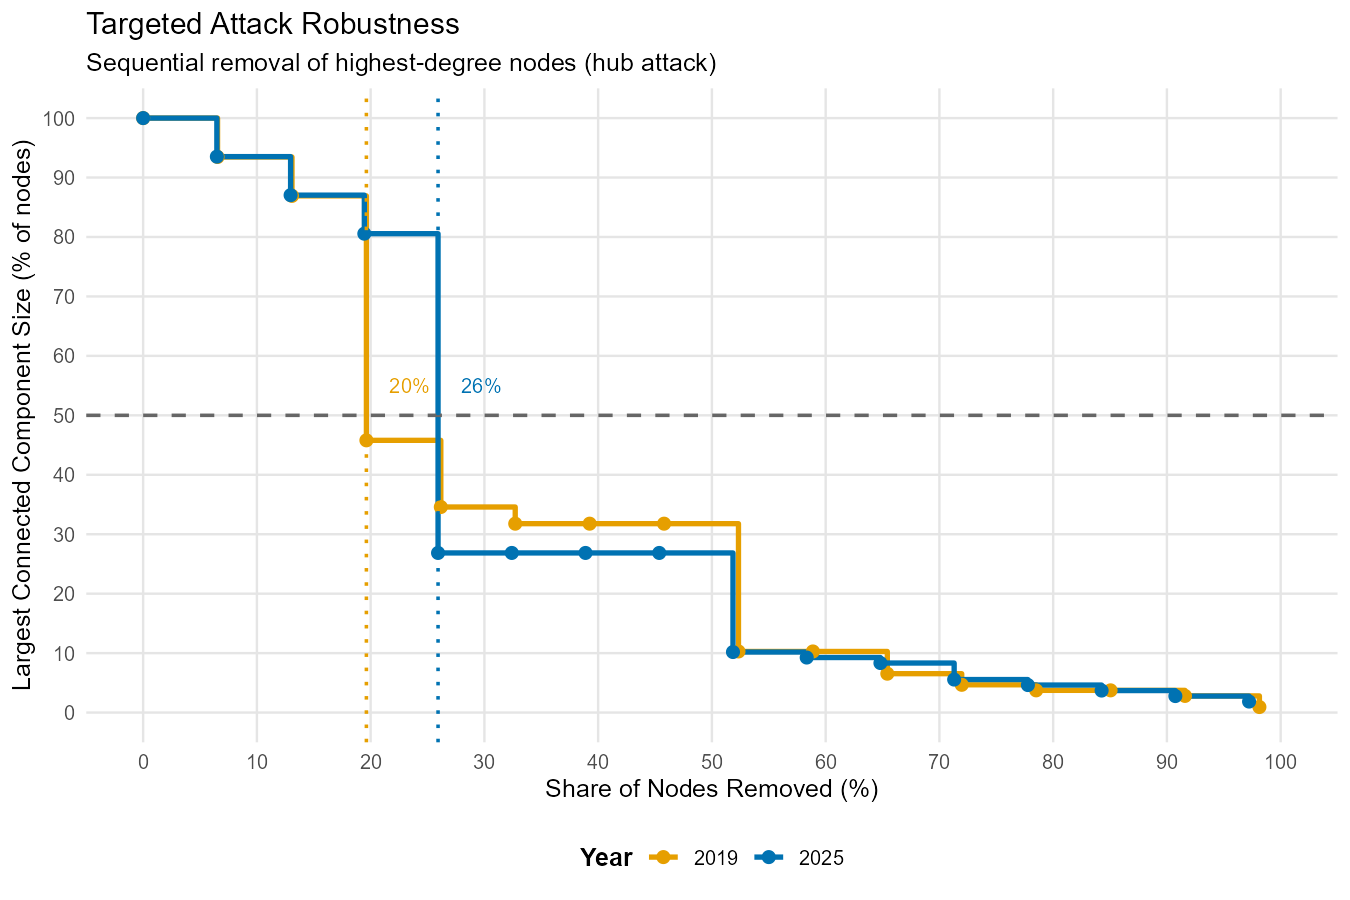
\includegraphics[width=0.85\textwidth]{robustness_targeted_attack.png}
  \caption{Robustness under targeted hub removal.
  Nodes are removed iteratively in descending degree order and the relative size of the largest connected component (LCC) is tracked.
  The 2025 network drops below the 50\,\% LCC threshold after removing 26\,\% of nodes, compared to 20\,\% in 2019, indicating slightly higher robustness against hub-focused disruptions in the transfer-based connectivity model.}\label{fig:targeted}
\end{figure}

\begin{figure}[htbp]
  \centering
  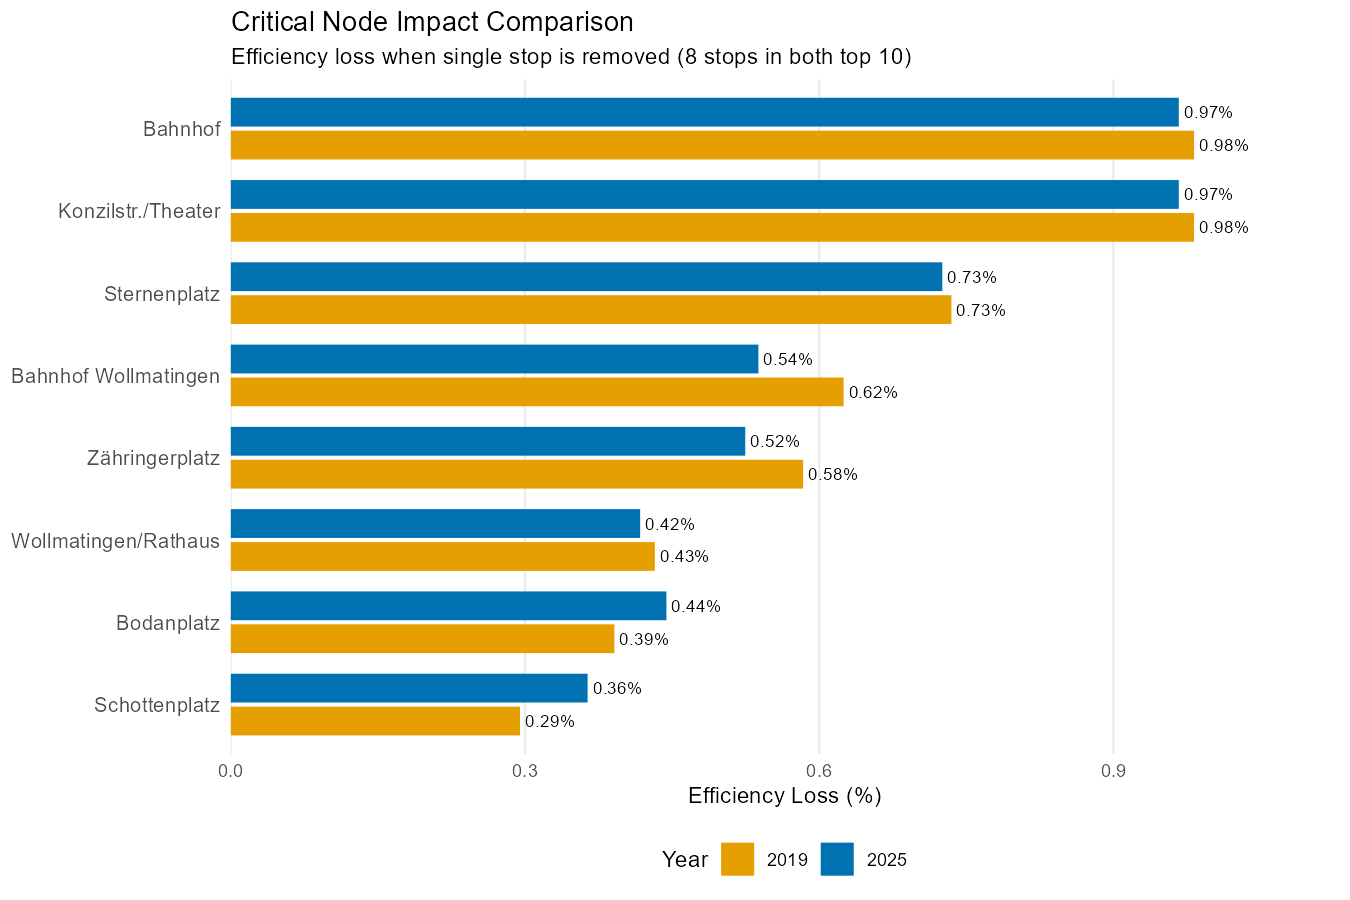
\includegraphics[width=0.85\textwidth]{robustness_critical_nodes.png}
  \caption{Critical stops under single-node removal.
  Bars show the efficiency loss (\%) after removing the same stop from the transfer-based reachability network.
  Bahnhof, Konzilstr./Theater, and Sternenplatz remain the most critical in both years.
  Stops that appear only in one year's top~10 are discussed in the text.}\label{fig:critical}
\end{figure}

Under random failures, efficiency remains almost unchanged at 20~percent random removal.
In 2019, average efficiency at 20~percent removal is 0.6522, which corresponds to 99.8~percent of the baseline.
In 2025, average efficiency at 20~percent removal is 0.6579, which rounds to 100.0~percent of the baseline.
Overall, the robustness simulations suggest slightly higher robustness in 2025, although the differences are small in absolute terms, which is consistent with the generally dense transfer-free adjacency representation.

\section{Stop additions and removals}\label{sec:stop-changes}

In addition to changes among common stops, the stop set itself changes slightly.
Three stops present in 2019 are not present in the 2025 dataset: Lutherplatz, Tenbrinkstra\ss{}e, and Sonnenb\"{u}hlstra\ss{}e/Tannenhof.
Four stops appear only in 2025: Klingenbergstra\ss{}e, Ebertplatz, Buhlenweg~S\"{u}d, and Stephansschule.

These changes likely reflect a combination of service restructuring and stop-level adjustments.
Because stop names were harmonised across years, these additions and removals are interpreted as substantive differences rather than naming artefacts.
The year-to-year comparison therefore captures both rewiring among common stops and small changes in network coverage through stop additions and removals.

\section{Summary of main findings}\label{sec:results-summary}

The results show a slightly denser and more clustered transfer-free reachability network in 2025 compared to 2019, with marginally shorter average shortest paths and a stable overall diameter.
The most central hubs and bottlenecks remain largely unchanged at the very top, indicating structural stability of the network core.
At the same time, a sizable set of stop pairs gains direct transfer-free connectivity while another set loses it, and most stops experience non-zero changes in their direct reachability.
This combination of stability at the core and rewiring in the periphery suggests that the timetable change between 2019 and 2025 produces meaningful redistribution of direct connectivity rather than a fundamental transformation of the network's central skeleton.

% ═══════════════════════════════════════════════════════════════════════════════
%  CHAPTER 6 — Discussion
% ═══════════════════════════════════════════════════════════════════════════════
\chapter{Discussion}\label{ch:discussion}

\section{Interpreting the structural change from 2019 to 2025}\label{sec:interp}

The comparison of the 2019 and 2025 timetable versions shows a combination of stability in the network core and noticeable rewiring in transfer-free connectivity.
On the one hand, global connectivity increases slightly.
The 2025 network has more transfer-free stop pairs, higher density, and higher clustering, alongside a marginally shorter average shortest path length.
On the other hand, the pair-level comparison reveals that this net increase is produced by substantial offsetting change.
A large set of connections is newly gained while another set is removed, and most stops experience non-zero net changes.

From a network-theoretical perspective, this pattern fits well with the idea that transport systems often exhibit stable structural backbones shaped by enduring spatial and functional constraints, while still allowing meaningful reconfiguration at the periphery or along secondary corridors \citep{barthelemy2011}.
In Konstanz, the identity of the most central nodes remains highly stable across 2019 and 2025.
Bahnhof, Konzilstr./Theater, Sternenplatz, and Z\"{a}hringerplatz remain the dominant hubs and also the dominant bottlenecks when bottlenecks are interpreted through betweenness centrality.
This is consistent with the expectation that nodes associated with the main interchange area and the city centre continue to channel movement even when timetables change.

At the same time, secondary centrality shifts and the winners-and-losers analysis indicates redistribution.
Stops such as Bodan/Riedstra\ss{}e, Friedhof, and Bismarcksteig gain many new direct connections, while others such as Universit\"{a}t and Jacob-Burckhardt-Stra\ss{}e lose direct connectivity.
This combination suggests that the 2025 timetable does not fundamentally decentralise the network, but it does reallocate transfer-free reachability across particular locations.

A noteworthy structural signal is the decrease in maximum betweenness centrality from 2019 to 2025.
This is consistent with the robustness simulations.
The maximum single-node efficiency loss decreases slightly from 0.98~percent in 2019 to 0.97~percent in 2025, and the network withstands targeted hub removal for longer in 2025, reaching the 50~percent largest connected component threshold after removing 26~percent of nodes compared to 20~percent in 2019.
These differences are modest, but together they support the interpretation of a small reduction in dependence on the most central intermediaries.
At the same time, the robustness results should be interpreted as structural robustness in the transfer-based topological model, not as resilience to physical infrastructure disruptions.

\section{Hubs, bottlenecks, and what they mean in a transfer-based representation}\label{sec:hub-meaning}

This thesis operationalises a connection as transfer-free reachability.
As a result, hub status in this network is closely tied to the everyday experience of having many destinations reachable without changing buses.
Degree centrality is therefore directly interpretable as the number of direct destinations from a stop.
Betweenness centrality, computed on shortest paths in this binary network, is interpretable as transfer-based mediation.
Stops with high betweenness lie on many minimal-transfer paths, which aligns with an intuitive understanding of bottlenecks in a network where transfers are costly \citep{derrible2010}.

This representation connects to the literature on efficiency in timetable-based public transport networks.
\citet{gallotti2014} emphasise that network structure shapes detours and constraints in urban mobility.
Even without modelling travel times and service frequencies, the transfer-free connectivity network captures an important dimension of perceived convenience, because transfers are widely discussed as carrying an additional perceived burden for passengers \citep{iseki2009}.
The results suggest that the 2025 timetable slightly expands the possibility space of transfer-free travel overall, but the distribution of that benefit is uneven.

The prominence of a few central nodes in both years also aligns with broader insights on spatial networks, where geography and the organisation of urban functions often create highly central nodes that persist across time \citep{barthelemy2011}.
Konstanz appears to follow this pattern.
The main hubs remain stable, and changes are more pronounced in the surrounding structure.

\section{Practical implications and trade-offs}\label{sec:practical}

From a practical perspective, the results provide a clear summary of what changes in the network may feel like for users.
The global increase in transfer-free connections suggests that, on average, more destinations can be reached directly in 2025 than in 2019.
Higher clustering indicates that groups of stops become more mutually reachable without transfers, which can be interpreted as stronger local redundancy of direct links.

However, the winners-and-losers analysis shows that improvements are not uniform.
Some stops gain many new direct destinations, while others lose direct reachability.
The fact that Universit\"{a}t appears among the strongest losers is substantively relevant, because major trip generators are often expected to remain well connected.
This does not automatically mean that access to the university worsened in a broader sense.
A stop can lose direct connections while still remaining well served through one transfer.
Because transfers are often perceived as inconvenient, an increase in required transfers can matter for experienced service quality even when overall connectivity remains high \citep{iseki2009}.

This is an example of a broader trade-off typical for public transport planning in small and medium-sized cities.
Limited resources and limited redundancy can lead to designs that improve some direct connections at the expense of others, or that simplify lines and reduce coverage of certain direct links while maintaining overall connectivity through transfers \citep{cipriani2019}.
In that sense, the Konstanz comparison can be read as a concrete illustration of how structural constraints and planning decisions manifest in network metrics and transfer-free reachability.

The repeated appearance of Staad/Autof\"{a}hre in both gained and removed example pairs also suggests that the timetable revision may have reorganised connectivity around specific corridors or destinations.
Even when overall connectivity improves, a reconfiguration can create pronounced local changes that are highly visible to affected users.
The adjacency-based approach used here can therefore serve as a transparent tool for communication, because it allows planners or stakeholders to point to concrete pairs and concrete stops where transfer-free travel was gained or lost, without claiming to fully evaluate service quality.

\section{Limitations}\label{sec:limitations}

Several limitations follow directly from the design choices that make the analysis feasible and interpretable.

First, the data represent a snapshot of a typical weekday service situation in May around midday.
Public transport networks are time-dependent, and service patterns can differ by time of day, school periods, and weekends.
The chosen snapshot improves comparability between 2019 and 2025, but it does not represent the full timetable space.
This matters especially if some lines have strong peak-only variants or school runs.

Second, the analysis focuses on the bus network only and excludes cross-border services and certain special services.
This is consistent with the scope definition, but it implies that the results do not describe the full public transport system of Konstanz in a multimodal sense.
Multilayer and multimodal research shows that integrating modes can change conclusions about accessibility and vulnerability \citep{alessandretti2022}.
The findings should therefore be interpreted as statements about the bus network snapshot, not about the entire mobility system.

In addition, the robustness simulations treat node failures as independent events in an abstract topological network.
In reality, bus services share physical infrastructure such as bridges and arterial roads.
Failure of such infrastructure can induce correlated multi-stop and multi-route disruptions that are not captured by independent node removal.
A more complete resilience analysis would require an explicit spatial or route-based representation that links stops and lines to shared infrastructure elements, which is beyond the scope of this study.

Third, the adjacency definition treats all stop pairs served by the same line as directly connected and models the resulting relation as undirected.
This captures mutual transfer-free connectivity at the level of whether a direct ride is possible, but it abstracts from direction-specific stop patterns and from the possibility that some services do not serve all stops equally in both directions.
This simplification is acceptable for the thesis focus, but it may slightly overstate connectivity in cases where directionality matters.

Fourth, the network is binary and unweighted.
It does not incorporate service frequency, travel time, waiting time, or reliability.
As a result, the measures capture the existence of transfer-free options rather than how attractive those options are.
This matters because a rare direct ride might be less useful than a frequent one-transfer alternative.
The analysis therefore addresses structural connectivity and transfer requirements, not generalised travel cost.

Fifth, the datasets were manually digitised.
Although plausibility checks and harmonisation were applied, manual transcription can introduce error.
This limitation is partly offset by the interpretability of the pipeline and by the fact that the key results are pattern-based and would require systematic errors to change qualitatively.

Finally, the before--after design does not establish causality in a strict sense, because many contextual factors can change between 2019 and 2025, including demand patterns, construction, and planning priorities.
The analysis therefore supports descriptive and theory-informed interpretation of structural change rather than causal claims about policy effectiveness.

\section{Implications for future research}\label{sec:future}

Several extensions would deepen the theoretical and practical value of the analysis while remaining compatible with the network framework.

A first extension is a temporal or frequency-weighted representation.
Using edge weights based on number of departures or typical travel times would bring the analysis closer to efficiency concepts discussed in the literature on timetable-based networks \citep{gallotti2014}.
A second extension is to incorporate directionality explicitly and to compare results under symmetric versus directional definitions of direct connectivity.
A third extension is to move from independent node failures toward correlated disruption scenarios, for example by removing complete lines, removing sets of stops that share a corridor, or approximating bridge or arterial-road outages through structured multi-node removals.
This would connect the robustness concept more directly to shared infrastructure dependencies.
A fourth extension is to move toward a multimodal framework that includes ferry or rail layers, which would connect directly to multilayer transport network perspectives \citep{alessandretti2022,artime2022}.

Taken together, these extensions would allow the core insights of this thesis to be tested for robustness and expanded toward richer operational and multimodal interpretations.
Within the scope of the present work, the comparison already demonstrates that even a simple transfer-free reachability model can reveal meaningful structural change and clear distributional patterns of gains and losses between timetable versions.

% ═══════════════════════════════════════════════════════════════════════════════
%  CHAPTER 7 — Conclusion and outlook
% ═══════════════════════════════════════════════════════════════════════════════
\chapter{Conclusion and outlook}\label{ch:conclusion}

\section{Answering the research question}\label{sec:answer}

This thesis asked how the public transport network in Konstanz is structured, which hubs and bottlenecks can be identified, and how these features change between the 2019 and 2025 timetable versions.
Using a transfer-free reachability representation, the results show a network with a stable core and meaningful redistribution at the margins.

First, the overall structure becomes slightly more connected in 2025.
The number of transfer-free connections increases, network density and clustering rise, and average shortest path length decreases marginally.
Interpreted in this framework, the 2025 timetable offers slightly more direct reachability without transfers and a modest increase in local redundancy of direct connections.

Second, the identity of the most central hubs and bottlenecks remains highly stable.
Bahnhof and the central stops around the city centre consistently rank at the top for both degree and betweenness.
This indicates that timetable change did not alter the central skeleton of the network.
Instead, it mainly reshaped connectivity around secondary nodes and corridors.

Third, the comparison reveals substantial rewiring beneath the stable core.
A large number of stop pairs gain direct connectivity while another set loses it, with most stop-level profiles changing.
The winners-and-losers analysis shows that gains and losses are unevenly distributed across stops.
Some locations gain many new direct connections, while others, including Universit\"{a}t, lose direct transfer-free reachability to multiple destinations.
This highlights a key practical implication of the timetable change.
Even when global connectivity improves, some users or areas can experience a higher transfer burden.

Overall, the Konstanz bus network in 2019 and 2025 can be characterised as a highly connected network with very short average path lengths and relatively high clustering in the transfer-based representation.
The structure is centred on a persistent core of hubs, with timetable revisions producing measurable shifts in where direct connectivity is concentrated and where it is reduced.
This directly answers the research question by showing both structural stability at the core and structural change in transfer-free reachability patterns.

\section{Outlook}\label{sec:outlook}

Several extensions would strengthen the theoretical and practical reach of the analysis.
First, a frequency-weighted or time-weighted network would move beyond the binary existence of a direct connection.
This would allow the analysis to distinguish frequent direct links from rare ones and to approximate travel cost more realistically, while still remaining within a network framework.

Second, a temporal extension could compare peak and off-peak snapshots or examine weekday versus weekend structures.
This would address the time dependence of transit systems and clarify whether the observed changes are stable across time windows.

Third, directionality could be incorporated explicitly.
Even if the main analysis remains undirected for interpretability, a robustness check with directed connections would strengthen the methodological argument and reduce the risk that one-way service patterns are masked.

Fourth, robustness could be extended beyond independent node failures toward correlated disruptions that reflect shared infrastructure and route interdependencies.
For example, removing complete routes or simulating corridor-level outages would better approximate disruptions such as bridge closures or long-lasting road works, which can affect multiple stops and lines simultaneously.

Fifth, the analysis could be expanded toward a multimodal representation, for example by adding ferry or rail layers, which would connect to broader multilayer transport perspectives.
Alternatively, demand data or passenger counts could be used to weight network elements, shifting the focus from structural possibility to likely usage.

Finally, an agent-based simulation could be used as an optional illustration rather than the core method.
For example, agents could be assigned origin--destination pairs and simple routing rules to estimate how the distribution of transfers changes under the two timetable versions.
This would be most useful if kept deliberately simple and used to visualise consequences of structural change, not to claim behavioural realism.

% ---------------------------------------------------------------------------
%  AI tool use statement
% ---------------------------------------------------------------------------
\clearpage
\chapter*{AI tool use statement}
\addcontentsline{toc}{chapter}{AI tool use statement}

Generative AI tools were used to support writing and coding, not to generate empirical results.
ChatGPT \citep{openai2025} was used for language editing (grammar, readability, and flow) and for drafting and refining text structure.
GitHub Copilot \citep{github2025} was used for coding assistance (code completion and debugging suggestions) while implementing the analysis pipeline in R.
All data were manually digitised by the author from the official timetable booklet, and all analytical choices, computations, and interpretations were made and verified by the author.
AI-generated suggestions were reviewed critically, adapted where appropriate, and checked against the underlying data and the cited literature.
No external text was copied verbatim from AI outputs without revision and attribution.

% ---------------------------------------------------------------------------
%  Bibliography
% ---------------------------------------------------------------------------
\clearpage
\bibliography{references}

% ---------------------------------------------------------------------------
%  Declaration of authorship (Eigenständigkeitserklärung)
% ---------------------------------------------------------------------------
\clearpage
\chapter*{Eigenst\"{a}ndigkeitserkl\"{a}rung}
\addcontentsline{toc}{chapter}{Eigenst\"{a}ndigkeitserkl\"{a}rung}

Hiermit erkl\"{a}re ich, dass ich die vorliegende Arbeit selbstst\"{a}ndig verfasst und keine anderen als die angegebenen Quellen und Hilfsmittel benutzt habe.
Die Stellen der Arbeit, die anderen Quellen im Wortlaut oder dem Sinn nach entnommen wurden, sind durch Angaben der Herkunft kenntlich gemacht.
Dies gilt auch f\"{u}r Zeichnungen, Skizzen, bildliche Darstellungen sowie f\"{u}r Quellen aus dem Internet.

\vspace{2cm}
\noindent
\begin{tabular}{@{}p{6cm}p{6cm}@{}}
  \hrulefill & \hrulefill \\
  Ort, Datum & Unterschrift
\end{tabular}

\end{document}
